\subsection*{Problema 05}

\textbf{Enunciado:} Calcular la integral indefinida
\begin{align*}
\int \dfrac{x}{\sqrt{x} - 1} \, dx
\end{align*}

\textbf{Solución:} Siguiendo las indicaciones, aplicamos la sustitución $u = \sqrt{x}$. 
De aquí obtenemos que $x = u^2$ y el diferencial es:
\begin{align*}
dx = 2u \, du
\end{align*}

Sustituimos estas expresiones en la integral original:
\begin{align*}
I &= \int \dfrac{u^2}{u - 1} (2u \, du) \\
I &= 2 \int \dfrac{u^3}{u - 1} \, du
\end{align*}

El integrando es un cociente de polinomios donde el grado del numerador es mayor que el del denominador. Realizamos la división algebraica de $u^3$ entre $u - 1$. 

Dividiendo $u^3$ por $u - 1$:
\begin{align*}
\dfrac{u^3}{u - 1} = u^2 + u + 1 + \dfrac{1}{u - 1}
\end{align*}

Sustituimos este resultado en nuestra integral:
\begin{align*}
I &= 2 \int \left( u^2 + u + 1 + \dfrac{1}{u - 1} \right) du
\end{align*}

integramos término a término:
\begin{align*}
I &= 2 \left( \dfrac{u^3}{3} + \dfrac{u^2}{2} + u + \ln|u - 1| \right) + C
\end{align*}

Multiplicamos por el factor $2$:
\begin{align*}
I &= \dfrac{2}{3}u^3 + u^2 + 2u \\
&\quad + 2\ln|u - 1| + C
\end{align*}

Finalmente, regresamos a la variable original sustituyendo $u = \sqrt{x}$:
\begin{align*}
I &= \dfrac{2}{3}(\sqrt{x})^3 + (\sqrt{x})^2 \\
&\quad + 2\sqrt{x} + 2\ln|\sqrt{x} - 1| + C
\end{align*}

Simplificando los exponentes, el resultado final de la integral es:
\begin{align*}
\int \dfrac{x}{\sqrt{x} - 1} \, dx &= \dfrac{2}{3}x^{3/2} + x + 2\sqrt{x} \\
&\quad + 2\ln|\sqrt{x} - 1| + C
\end{align*}

\begin{figure}[H]
	\centering
	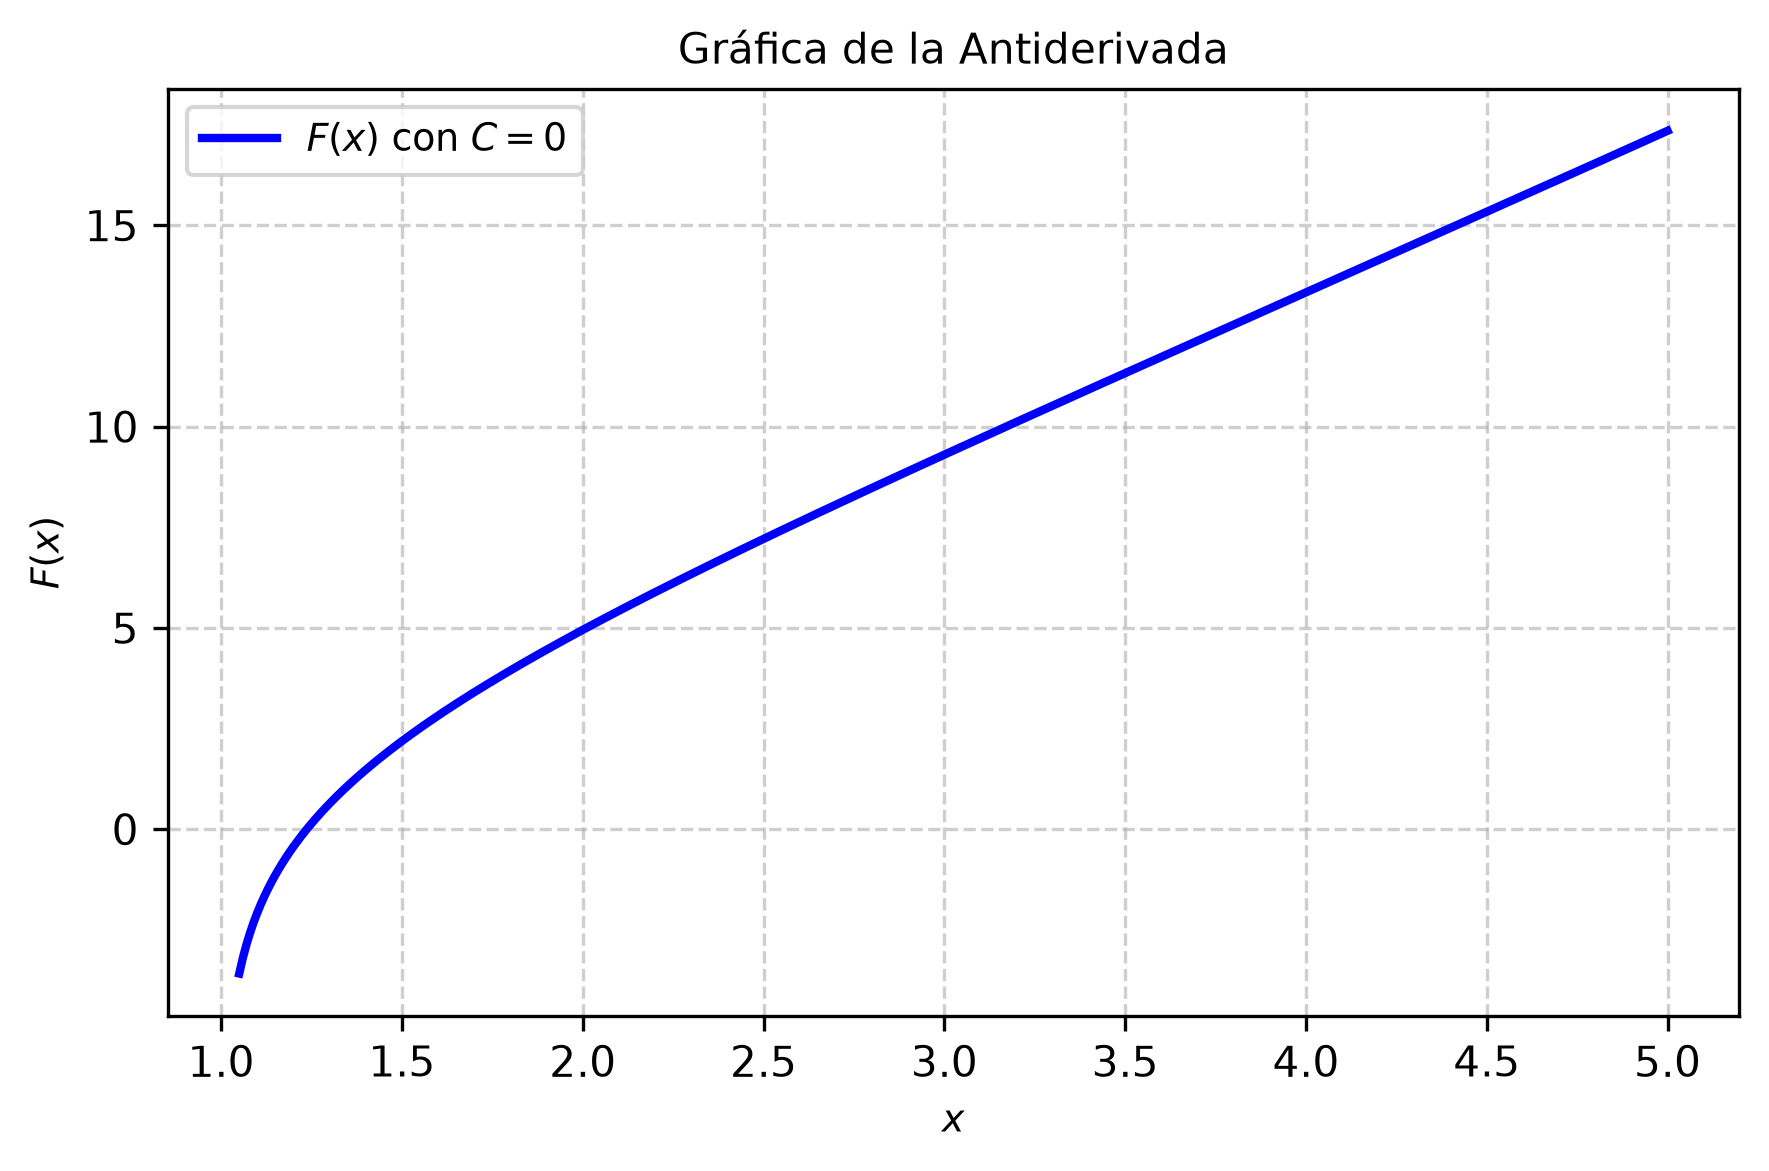
\includegraphics[width=\columnwidth]{semana_05/graficas/SEM05_P05_grafica.png}
	\caption{Representación gráfica de $f(x)$ y su antiderivada $F(x)$ evaluada para la constante de integración $C = 0$ (Problema 05).}
	\label{fig:problema05}
\end{figure}
